% Compile with xelatex if available:
% xelatex project_report_find_my_teammate.tex
% Fallback:
% pdflatex project_report_find_my_teammate.tex

\documentclass[12pt,a4paper,oneside]{report}

\usepackage[a4paper,left=1.5in,right=1in,top=1in,bottom=1in]{geometry}
\usepackage{iftex}
\ifPDFTeX
  \usepackage[T1]{fontenc}
  \usepackage[utf8]{inputenc}
  \usepackage{newtxtext,newtxmath}
\else
  \usepackage{fontspec}
  \setmainfont{Times New Roman}
\fi

\usepackage{setspace}
\usepackage{titlesec}
\usepackage{graphicx}
\usepackage{array}
\usepackage{booktabs}
\usepackage{longtable}
\usepackage{tabularx}
\usepackage{multirow}
\usepackage{ragged2e}
\usepackage{enumitem}
\usepackage{caption}
\usepackage{float}
\usepackage{pgfgantt}
\usepackage{tikz}
\usepackage{hyperref}
\usepackage{pdflscape}
\usepackage{verbatim}
\usepackage{fancyhdr}
\usetikzlibrary{arrows.meta,positioning,shapes.geometric,shapes.misc,fit,calc,matrix}

\hypersetup{
  colorlinks=true,
  linkcolor=black,
  urlcolor=blue,
  citecolor=black,
  pdftitle={Find My Teammate Project Report},
  pdfauthor={Faculty of Computer Applications}
}

\onehalfspacing
\setlength{\parindent}{0.5in}
\setlength{\parskip}{0.25em}
\setcounter{secnumdepth}{3}
\setcounter{tocdepth}{3}
\renewcommand{\arraystretch}{1.25}
\newcolumntype{Y}{>{\RaggedRight\arraybackslash}X}
\newcolumntype{L}[1]{>{\RaggedRight\arraybackslash}p{#1}}
\newcolumntype{C}[1]{>{\Centering\arraybackslash}p{#1}}
\setlength{\LTleft}{0pt}
\setlength{\LTright}{0pt}

\titleformat{\chapter}[display]
  {\bfseries\fontsize{16}{18}\selectfont\centering}
  {\MakeUppercase{Chapter \thechapter}}
  {0pt}
  {\vspace{0.5ex}\MakeUppercase}

\titleformat{\section}
  {\bfseries\fontsize{14}{16}\selectfont}
  {\thesection}
  {1em}
  {\MakeUppercase}

\titleformat{\subsection}
  {\bfseries\fontsize{12}{14}\selectfont}
  {\thesubsection}
  {1em}
  {}

\newcommand{\projecttitle}{Find My Teammate}
\newcommand{\reporttype}{A Major Project Report}
\newcommand{\degree}{Master of Computer Applications}
\newcommand{\sessionyear}{2025--2026}
\newcommand{\submissionmonthyear}{May 2026}
\newcommand{\supervisorname}{Dr./Prof. \underline{\hspace{1.8in}}}
\newcommand{\hodname}{Dr./Prof. \underline{\hspace{1.8in}}}
\newcommand{\internalexaminer}{Dr./Prof. \underline{\hspace{1.8in}}}
\newcommand{\externalexaminer}{Dr./Prof. \underline{\hspace{1.8in}}}
\newcommand{\studentone}{\textbf{Student Name 1}}
\newcommand{\rollone}{\textbf{Roll Number 1}}
\newcommand{\studenttwo}{\textbf{Student Name 2}}
\newcommand{\rolltwo}{\textbf{Roll Number 2}}
\newcommand{\organisationname}{\underline{\hspace{2.5in}}}
\newcommand{\industrymentor}{\underline{\hspace{2.5in}}}
\newcommand{\college}{Faculty of Computer Applications\\Acropolis Institute of Technology \& Research, Indore}

\newcommand{\signatureblock}[2]{
  \begin{minipage}[t]{0.45\textwidth}
    \centering
    \vspace{2em}
    \rule{2.2in}{0.4pt}\\
    #1\\
    #2
  \end{minipage}
}

\newcommand{\makecoverpage}{
  \begin{titlepage}
    \thispagestyle{empty}
    \begin{center}
      \vspace*{0.5cm}
      {\fontsize{24}{28}\selectfont\bfseries \projecttitle \par}
      \vspace{1.1cm}
      {\fontsize{14}{18}\selectfont\bfseries \reporttype \par}
      \vspace{0.9cm}
      {\fontsize{12}{16}\selectfont Submitted in Partial Fulfilment of the Requirements for the Award of the Degree of\par}
      \vspace{0.6cm}
      {\fontsize{14}{18}\selectfont\bfseries \MakeUppercase{\degree}\par}
      \vspace{1cm}
      \fbox{
        \begin{minipage}[c][3.0cm][c]{3.0cm}
          \centering
          \textbf{COLLEGE\\LOGO}
        \end{minipage}
      }
      \vspace{1cm}

      {\fontsize{12}{16}\selectfont Session: \sessionyear\par}
      \vspace{1cm}

      {\fontsize{14}{18}\selectfont\bfseries SUPERVISED BY\par}
      \vspace{0.4cm}
      {\fontsize{12}{16}\selectfont \supervisorname\par}
      \vspace{1cm}

      {\fontsize{14}{18}\selectfont\bfseries SUBMITTED BY\par}
      \vspace{0.5cm}
      \begin{tabular}{p{2.7in}p{2.1in}}
        \centering \textbf{Name of Student(s)} & \centering \textbf{Roll Number} \tabularnewline
        \studentone & \rollone \tabularnewline
        \studenttwo & \rolltwo \tabularnewline
      \end{tabular}

      \vfill
      {\fontsize{14}{18}\selectfont \college\par}
      \vspace{0.4cm}
      {\fontsize{14}{18}\selectfont \MakeUppercase{\submissionmonthyear}\par}
    \end{center}
  \end{titlepage}
}

\begin{document}

\makecoverpage
\makecoverpage

\pagenumbering{roman}

\chapter*{Certificate}
\addcontentsline{toc}{chapter}{Certificate}

This is to certify that this project report entitled ``\projecttitle'' submitted by \studentone\ (\rollone) and \studenttwo\ (\rolltwo) to \college\ in the partial fulfilment of the requirements for the degree of \degree\ during the academic session \sessionyear\ is a bona fide record of project work carried out by them under the supervision of \supervisorname.

\vspace{1em}
The work presented in this report is original and has not been submitted, either in full or in part, to any other university or institution for the award of any degree or diploma. In our opinion, the project work is satisfactory in scope, quality, and academic relevance for submission and evaluation.

\vspace{2em}
\noindent
\signatureblock{Signature of HOD}{\hodname}
\hfill
\signatureblock{Signature of Supervisor}{\supervisorname}

\vspace{3em}
\noindent
\signatureblock{Signature of External Examiner}{\externalexaminer}
\hfill
\signatureblock{Signature of Internal Examiner}{\internalexaminer}

\vspace{2em}
\noindent
\textbf{Date:} \underline{\hspace{1.4in}} \hfill \textbf{Place:} Indore

\chapter*{Internship Certificate}
\addcontentsline{toc}{chapter}{Internship Certificate}

This is to certify that \studentone\ (\rollone) and \studenttwo\ (\rolltwo) completed industrial exposure / internship / project training related to the development of ``\projecttitle'' at \organisationname\ under the guidance of \industrymentor.

\vspace{1em}
During the period of training, the students studied the requirements of collaboration platforms, analysed real user problems in team discovery, and implemented a prototype using React.js, Node.js, Express.js, MongoDB, JWT authentication, and Socket.IO for real-time features. Their conduct, technical learning, and project contribution were found satisfactory.

\vspace{3em}
\noindent
\signatureblock{Industry Mentor / Authorised Signatory}{\industrymentor}
\hfill
\signatureblock{Organisation Seal}{\organisationname}

\vspace{2em}
\noindent
\textbf{Date:} \underline{\hspace{1.4in}} \hfill \textbf{Place:} \underline{\hspace{1.4in}}

\chapter*{Acknowledgement}
\addcontentsline{toc}{chapter}{Acknowledgement}

We express our sincere gratitude to the Faculty of Computer Applications, Acropolis Institute of Technology \& Research, Indore for providing the academic environment, computing resources, and institutional support necessary for the completion of this project.

\vspace{0.5em}
We are deeply thankful to our project supervisor, \supervisorname, for continuous guidance, constructive feedback, and consistent encouragement throughout the analysis, design, implementation, and documentation stages of this work. Their suggestions helped us refine both the technical architecture and the academic presentation of the project.

\vspace{0.5em}
We also acknowledge the Head of Department, \hodname, and all faculty members of the department for their support, valuable inputs, and motivation during the semester. We thank our classmates, friends, and family members for their assistance during testing, feedback collection, and improvement of the user experience.

\vspace{0.5em}
Finally, we acknowledge all open-source communities and official documentation sources of React, Node.js, MongoDB, Express, Socket.IO, and related tools that made this project technically feasible and academically enriching.

\chapter*{Abstract}
\addcontentsline{toc}{chapter}{Abstract}

The project ``\projecttitle'' is a full-stack web application designed to solve the common problem of finding suitable teammates for hackathons, academic projects, startup ideas, and freelance collaborations. In many institutions and developer communities, students and professionals possess relevant technical skills but fail to identify reliable collaborators within limited time. The proposed system provides a unified digital platform where users can create a profile, display skills and interests, post project opportunities, discover teammates, send and manage collaboration requests, exchange messages in real time, and monitor activity through dashboards and notifications.

\vspace{0.5em}
The system has been implemented using the MERN technology stack. The frontend is built with React.js, Tailwind CSS, Axios, and React Router. The backend is developed using Node.js and Express.js with MongoDB as the database and Mongoose as the object modelling layer. Authentication is handled using JSON Web Tokens and secure password hashing with bcrypt. Real-time chat, online presence, and typing indication are supported using Socket.IO.

\vspace{0.5em}
The major contribution of the project lies in integrating teammate discovery, project posting, request handling, and communication within a single responsive platform. The application improves project formation speed, reduces coordination friction, and offers role-based features for normal users, team leads, and administrators. The proposed platform demonstrates practical full-stack development, database design, software engineering documentation, and system testing in a real-world academic context.

\tableofcontents
\listoftables
\listoffigures

\chapter*{List of Symbols and Abbreviations}
\addcontentsline{toc}{chapter}{List of Symbols and Abbreviations}

{\small
\setlength{\tabcolsep}{4pt}
\begin{longtable}{L{1.2in}L{4.05in}}
\toprule
\textbf{Abbreviation} & \textbf{Meaning} \\
\midrule
API & Application Programming Interface \\
CRUD & Create, Read, Update, Delete \\
DFD & Data Flow Diagram \\
ER Diagram & Entity Relationship Diagram \\
HTML & HyperText Markup Language \\
HTTP & HyperText Transfer Protocol \\
JWT & JSON Web Token \\
MCA & Master of Computer Applications \\
MERN & MongoDB, Express.js, React.js, Node.js \\
MVC & Model View Controller \\
REST & Representational State Transfer \\
UI & User Interface \\
UML & Unified Modeling Language \\
UX & User Experience \\
\bottomrule
\end{longtable}
}

\clearpage
\pagenumbering{arabic}

\chapter{Introduction}

\section{General Description of Project}
\projecttitle\ is a modern collaboration platform created for students, developers, and freelancers who need to find suitable teammates for technical and non-technical projects. In practical academic environments, project success often depends not only on an individual's idea but also on the timely availability of capable collaborators. However, team formation is frequently unstructured, informal, and inefficient. Students rely on classroom announcements, social media groups, or personal contacts, which often leads to delays, uneven distribution of skills, and poor communication.

The proposed system transforms this fragmented process into a structured digital workflow. Users register securely, complete a skill-based profile, browse open opportunities, publish project requirements, invite teammates, apply to existing projects, and communicate through a real-time messaging interface. The platform supports both one-to-one communication and project-driven interaction, making it suitable for hackathons, internships, course projects, research prototypes, and startup idea validation.

From a software engineering perspective, the project also demonstrates practical implementation of a full-stack architecture using modular frontend and backend layers. It integrates authentication, profile management, routing, API design, database schema design, request state management, and socket-based real-time features into one cohesive system.

\section{Objective}
The major objectives of the project are as follows:
\begin{enumerate}[label=\arabic*.]
  \item To build a centralised platform for identifying teammates based on skills, interests, and availability.
  \item To enable users to post project opportunities and define the specific skills required for collaboration.
  \item To provide a structured request workflow for joining projects and inviting teammates.
  \item To enable real-time communication using Socket.IO for immediate coordination and follow-up.
  \item To maintain dashboards, notifications, and administrative oversight for better usability and control.
  \item To demonstrate end-to-end full-stack software development using the MERN stack.
\end{enumerate}

\section{Scope}
The scope of the current version of \projecttitle\ includes:
\begin{itemize}
  \item User registration, login, and JWT-based session handling.
  \item Profile creation with skills, interests, biography, availability, and profile image.
  \item Project creation, browsing, filtering, bookmarking, and detailed project views.
  \item Join requests and lead-driven teammate invitations.
  \item Team management, including request approval and teammate removal by lead/admin.
  \item Real-time direct messaging with typing indication and presence status.
  \item Notification handling and unread state tracking.
  \item Responsive web interface and role-based administrative overview.
\end{itemize}

The current scope excludes video conferencing, AI-based skill matching, payment processing, and native mobile deployment. These features remain part of the future enhancement roadmap.

\chapter{Study of Existing System / Specification System Requirements}

\section{Preliminary Investigation and Identification of Need}
The project idea emerged from repeated observations in academic settings where students struggled to form balanced teams despite having relevant skills in programming, design, testing, documentation, or presentation. Discussions with peers indicated that team formation delays reduce available development time and often force students into unproductive groups.

To understand the need, common existing practices were studied:
\begin{itemize}
  \item WhatsApp and Telegram groups used for announcements.
  \item Classroom notice circulation and word-of-mouth communication.
  \item Generic social networking platforms such as LinkedIn and Discord.
  \item Freelance or portfolio sites that are not focused on academic team formation.
\end{itemize}

These platforms help people connect, but they do not provide a dedicated workflow for project opportunity posting, skill-based matching, project-specific invitation handling, and structured real-time collaboration.

\subsection{Existing System and Its Limitations}
The existing informal system suffers from several limitations:
\begin{enumerate}[label=\arabic*.]
  \item \textbf{Lack of structured discovery:} There is no reliable way to search teammates by skill combinations such as React + Node.js + UI design.
  \item \textbf{No project-specific workflow:} Users cannot directly relate a conversation to a specific project opportunity and its required skill set.
  \item \textbf{Poor visibility of availability:} Many team members appear interested but may not actually be available or committed.
  \item \textbf{No unified request management:} Join requests, invites, approvals, and rejections are managed manually and often get lost.
  \item \textbf{Communication fragmentation:} Messages occur across multiple platforms and cannot be tracked in relation to the project.
  \item \textbf{No central dashboard:} Team leads and users do not get consolidated views of active projects, invitations, and pending requests.
  \item \textbf{Weak auditability:} It becomes difficult to know who initiated a request, when it was accepted, and whether the person actually became part of the team.
  \item \textbf{Limited academic usability:} Generic platforms do not align with semester project workflows, supervision expectations, and project documentation needs.
\end{enumerate}

\subsection{Problem Statement}
There is a need for a dedicated web-based system that allows users to discover project opportunities, find collaborators based on skills, manage invitations and join requests, and communicate in real time within a unified project-centric environment.

\section{Requirement Specification}
\subsection{Specific Objective 1}
To provide a searchable digital ecosystem where users can publish their skills, browse open team opportunities, and discover potential collaborators using project-specific criteria.

\subsection{Specific Objective 2}
To establish a controlled collaboration workflow consisting of authentication, project posting, teammate invitations, join requests, approval/rejection, direct communication, and notification-driven follow-up.

\subsection{Detailed Requirement Summary}
\begin{table}[H]
\centering
\caption{Summary of Core Requirements}
\begin{tabularx}{\textwidth}{p{1.0in}Y Y}
\toprule
\textbf{Type} & \textbf{Requirement} & \textbf{Purpose} \\
\midrule
Functional & User registration, login, and profile management & Identify users securely and maintain skill-based records \\
Functional & Project creation and browsing & Allow leads to post requirements and users to find opportunities \\
Functional & Join requests and invitations & Support formal team formation workflows \\
Functional & Direct chat and notifications & Enable coordination and prompt status awareness \\
Functional & Dashboard and admin panel & Provide monitoring, control, and consolidated views \\
Non-functional & Responsive interface & Ensure accessibility on desktop and mobile devices \\
Non-functional & Security & Protect credentials, access rights, and API requests \\
Non-functional & Scalability & Support increasing users, projects, and messages \\
Non-functional & Maintainability & Ensure modular architecture and reusable components \\
\bottomrule
\end{tabularx}
\end{table}

\chapter{Project Planning}

\section{Project Schedule for Project Phases}
The project was divided into major phases to ensure disciplined implementation and timely completion. The planning followed an incremental model where each completed phase was validated before moving to the next one.

\begin{table}[H]
\centering
\caption{Project Phase Schedule}
{\small
\setlength{\tabcolsep}{4pt}
\begin{tabularx}{\textwidth}{C{0.45in}Y C{0.75in} C{0.75in} C{0.9in}}
\toprule
\textbf{S.No.} & \textbf{Phase} & \textbf{Start} & \textbf{End} & \textbf{Duration} \\
\midrule
1 & Problem identification and requirement gathering & Week 1 & Week 2 & 2 weeks \\
2 & Literature study and system planning & Week 3 & Week 4 & 2 weeks \\
3 & Database and API design & Week 5 & Week 6 & 2 weeks \\
4 & Frontend interface development & Week 7 & Week 9 & 3 weeks \\
5 & Backend module implementation & Week 8 & Week 11 & 4 weeks \\
6 & Real-time communication integration & Week 12 & Week 13 & 2 weeks \\
7 & Testing and bug fixing & Week 14 & Week 15 & 2 weeks \\
8 & Documentation and report preparation & Week 16 & Week 18 & 3 weeks \\
\bottomrule
\end{tabularx}
}
\end{table}

\section{Gantt Chart (Timeline of Project Phases)}
\begin{figure}[H]
\centering
\resizebox{\linewidth}{!}{%
\begin{ganttchart}[
  x unit=0.30cm,
  y unit chart=0.52cm,
  title height=1,
  vgrid,
  hgrid,
  bar/.append style={fill=gray!50},
  title/.append style={fill=gray!15},
  bar label font=\footnotesize,
  title label font=\footnotesize
]{1}{18}
\gantttitle{Project Weeks}{18} \\
\gantttitlelist{1,...,18}{1} \\
\ganttbar{Requirement Gathering}{1}{2} \\
\ganttbar{Planning and Feasibility}{3}{4} \\
\ganttbar{Database Design}{5}{6} \\
\ganttbar{API and Backend Modules}{7}{11} \\
\ganttbar{Frontend Development}{7}{10} \\
\ganttbar{Chat and Socket Integration}{12}{13} \\
\ganttbar{Testing and Debugging}{14}{15} \\
\ganttbar{Documentation and Final Review}{16}{18}
\end{ganttchart}%
}
\caption{Indicative Gantt Chart for Development Phases}
\end{figure}

\chapter{System Analysis}

\section{Hardware Requirement}
\begin{table}[H]
\centering
\caption{Hardware Requirements}
\begin{tabularx}{\textwidth}{p{2.3in}Y}
\toprule
\textbf{Component} & \textbf{Specification} \\
\midrule
Processor & Intel Core i5 or equivalent / AMD Ryzen 5 or above \\
RAM & Minimum 8 GB (16 GB recommended for smoother local development) \\
Storage & 20 GB free space for source code, dependencies, and local database \\
Network & Broadband internet connection for package installation and cloud deployment \\
Display & 1366 x 768 resolution or above for effective UI testing \\
Input devices & Keyboard, mouse, and optional smartphone for responsive testing \\
\bottomrule
\end{tabularx}
\end{table}

\section{Software Requirement}
\begin{table}[H]
\centering
\caption{Software Requirements}
\begin{tabularx}{\textwidth}{p{2.3in}Y}
\toprule
\textbf{Software} & \textbf{Purpose} \\
\midrule
Windows 10/11 or Linux & Development operating system \\
Node.js and npm & Runtime and package management for client and server \\
React.js and Vite & Frontend development and bundling \\
Express.js & REST API implementation \\
MongoDB and Mongoose & NoSQL database and schema modelling \\
Socket.IO & Real-time messaging and presence updates \\
VS Code & Source code editing \\
Git and GitHub & Version control and collaboration \\
Postman / Thunder Client & API testing \\
Google Chrome / Edge & Browser testing and debugging \\
\bottomrule
\end{tabularx}
\end{table}

\section{System Analysis Tools}

\subsection{E-R Diagram}
\begin{figure}[H]
\centering
\resizebox{\linewidth}{!}{%
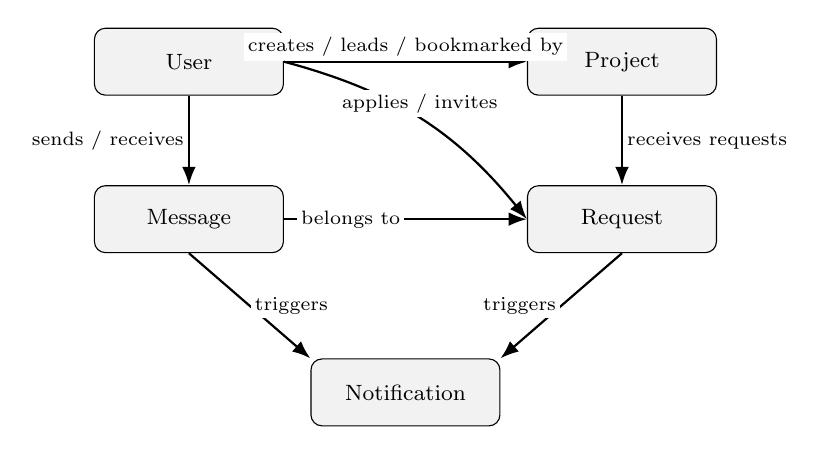
\begin{tikzpicture}[
  every node/.style={font=\footnotesize},
  entity/.style={draw, rounded corners, minimum width=2.4cm, minimum height=0.85cm, align=center, fill=gray!10},
  rel/.style={-Latex, thick},
  note/.style={font=\scriptsize, fill=white, inner sep=1.5pt}
]
\node[entity] (user) at (0,2.0) {User};
\node[entity] (project) at (5.5,2.0) {Project};
\node[entity] (message) at (0,0) {Message};
\node[entity] (request) at (5.5,0) {Request};
\node[entity] (notification) at (2.75,-2.2) {Notification};

\draw[rel] (user) -- node[note, above] {creates / leads / bookmarked by} (project);
\draw[rel] (user) -- node[note, left] {sends / receives} (message);
\draw[rel] (project) -- node[note, right] {receives requests} (request);
\draw[rel] (user.east) to[bend left=18] node[note, above] {applies / invites} (request.west);
\draw[rel] (message) -- node[note, left] {belongs to} (request);
\draw[rel] (message.south) -- node[note, right] {triggers} (notification.north west);
\draw[rel] (request.south) -- node[note, left] {triggers} (notification.north east);
\end{tikzpicture}%
}
\caption{High-Level Entity Relationship Diagram}
\end{figure}

\subsection{Data Flow Diagram}
\begin{figure}[H]
\centering
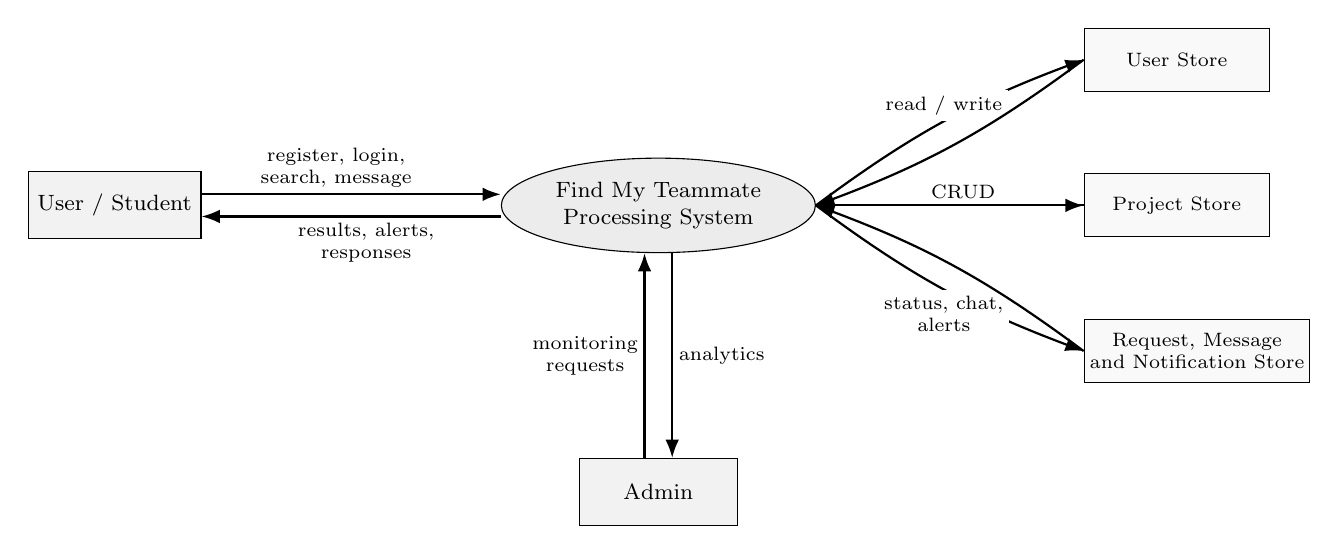
\begin{tikzpicture}[
  font=\footnotesize,
  node distance=1.9cm and 3.6cm,
  ext/.style={draw, minimum width=2.0cm, minimum height=0.85cm, fill=gray!10, align=center},
  proc/.style={draw, ellipse, minimum width=3.2cm, minimum height=1.2cm, fill=gray!15, align=center, inner sep=3pt},
  store/.style={draw, minimum width=2.35cm, minimum height=0.8cm, fill=gray!05, align=center, font=\scriptsize, inner sep=2pt},
  flow/.style={-Latex, thick},
  note/.style={font=\scriptsize, fill=white, inner sep=2pt}
]
\node[ext] (student) {User / Student};
\node[proc, right=3.8cm of student] (system) {\projecttitle\\Processing System};
\node[store, right=3.4cm of system, yshift=1.85cm] (db1) {User Store};
\node[store, right=3.4cm of system] (db2) {Project Store};
\node[store, right=3.4cm of system, yshift=-1.85cm] (db3) {Request, Message\\and Notification Store};
\node[ext, below=2.6cm of system] (admin) {Admin};

\draw[flow] ([yshift=4pt]student.east) -- node[note, above, pos=0.45, align=center] {register, login,\\search, message} ([yshift=4pt]system.west);
\draw[flow] ([yshift=-4pt]system.west) -- node[note, below, pos=0.45, align=center] {results, alerts,\\responses} ([yshift=-4pt]student.east);
\draw[flow] (system.east) to[bend left=8] node[note, above, pos=0.5] {read / write} (db1.west);
\draw[flow] (db1.west) to[bend left=8] (system.east);
\draw[flow] (system.east) -- node[note, above, pos=0.55] {CRUD} (db2.west);
\draw[flow] (db2.west) -- (system.east);
\draw[flow] (system.east) to[bend right=8] node[note, below, pos=0.5, align=center] {status, chat,\\alerts} (db3.west);
\draw[flow] (db3.west) to[bend right=8] (system.east);
\draw[flow] ([xshift=-5pt]admin.north) -- node[note, left, pos=0.5, align=center] {monitoring\\requests} ([xshift=-5pt]system.south);
\draw[flow] ([xshift=5pt]system.south) -- node[note, right, pos=0.5] {analytics} ([xshift=5pt]admin.north);
\end{tikzpicture}
\caption{Level-0 Data Flow Diagram}
\end{figure}

\subsection{Use Case}
\begin{figure}[H]
\centering
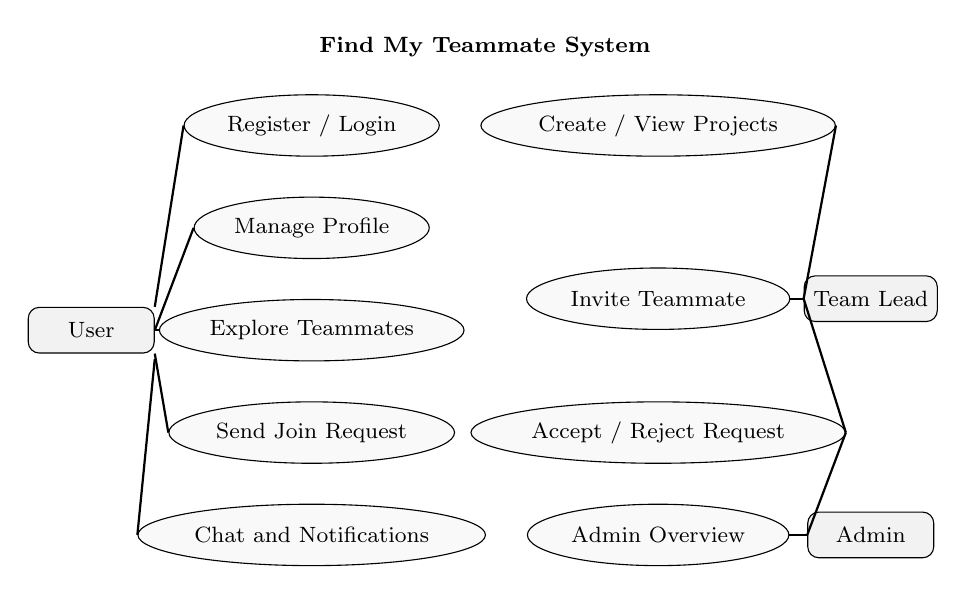
\begin{tikzpicture}[
  font=\footnotesize,
  actor/.style={draw, rounded corners, minimum width=1.6cm, minimum height=0.58cm, fill=gray!10, align=center},
  usecase/.style={draw, ellipse, minimum width=2.7cm, minimum height=0.78cm, fill=gray!05, align=center, inner sep=2pt},
  assoc/.style={thick}
]
% Use cases without boundary box
\node[font=\footnotesize\bfseries] at (6.0,3.8) {Find My Teammate System};

\node[usecase] (u1) at (3.8,2.8) {Register / Login};
\node[usecase] (u2) at (3.8,1.5) {Manage Profile};
\node[usecase] (u3) at (3.8,0.2) {Explore Teammates};
\node[usecase] (u5) at (3.8,-1.1) {Send Join Request};
\node[usecase] (u4) at (3.8,-2.4) {Chat and Notifications};

\node[usecase] (u6) at (8.2,2.8) {Create / View Projects};
\node[usecase] (u7) at (8.2,0.6) {Invite Teammate};
\node[usecase] (u8) at (8.2,-1.1) {Accept / Reject Request};
\node[usecase] (u9) at (8.2,-2.4) {Admin Overview};

% Actors
\node[actor] (user) at (1.0,0.2) {User};
\node[actor] (lead) at (10.9,0.6) {Team Lead};
\node[actor] (admin) at (10.9,-2.4) {Admin};

% User associations
\draw[assoc] (user.north east) -- (u1.west);
\draw[assoc] (user.east) -- (u2.west);
\draw[assoc] (user.east) -- (u3.west);
\draw[assoc] (user.south east) -- (u5.west);
\draw[assoc] ([yshift=-2pt]user.south east) -- (u4.west);

% Team Lead associations
\draw[assoc] (lead.west) -- (u6.east);
\draw[assoc] (lead.west) -- (u7.east);
\draw[assoc] (lead.west) -- (u8.east);

% Admin associations
\draw[assoc] (admin.west) -- (u9.east);
\draw[assoc] (admin.west) -- (u8.east);
\end{tikzpicture}
\caption{Use Case Diagram}
\end{figure}

\subsection{Activity Diagram}
\begin{figure}[H]
\centering
\resizebox{0.95\linewidth}{!}{%
\begin{tikzpicture}[
  every node/.style={font=\footnotesize},
  step/.style={draw, rounded corners, minimum width=4.8cm, minimum height=0.8cm, fill=gray!08, align=center},
  decision/.style={draw, diamond, aspect=2.4, inner xsep=0.6em, inner ysep=0.8em, align=center, fill=gray!08, font=\scriptsize},
  arrow/.style={-Latex, thick}
]
\node[step] (start) {Start and Open Platform};
\node[step, below=0.85cm of start] (login) {Register / Login};
\node[step, below=0.85cm of login] (browse) {Browse Projects or Explore Teammates};
\node[decision, below=1.0cm of browse] (choose) {Create project\\or join existing?};
\node[step, below left=1.2cm and 2.2cm of choose] (create) {Create Project Post};
\node[step, below right=1.2cm and 2.2cm of choose] (request) {Send Request /\\Accept Invite};
\node[step, below=2.6cm of choose] (approve) {Lead Reviews Request};
\node[step, below=0.85cm of approve] (chat) {Users Start Real-Time Chat};
\node[step, below=0.85cm of chat] (dash) {Track Progress from Dashboard};
\node[step, below=0.85cm of dash] (end) {End};

\draw[arrow] (start) -- (login);
\draw[arrow] (login) -- (browse);
\draw[arrow] (browse) -- (choose);
\draw[arrow] (choose.west) -- node[above left, font=\scriptsize] {Post} (create.north);
\draw[arrow] (choose.east) -- node[above right, font=\scriptsize] {Apply} (request.north);
\draw[arrow] (create.south) |- ([xshift=-0.7cm]approve.west) -- (approve.west);
\draw[arrow] (request.south) |- ([xshift=0.7cm]approve.east) -- (approve.east);
\draw[arrow] (approve) -- (chat);
\draw[arrow] (chat) -- (dash);
\draw[arrow] (dash) -- (end);
\end{tikzpicture}%
}
\caption{Activity Diagram for Team Formation Workflow}
\end{figure}

\subsection{State Diagram}
\begin{figure}[H]
\centering
\resizebox{0.88\linewidth}{!}{%
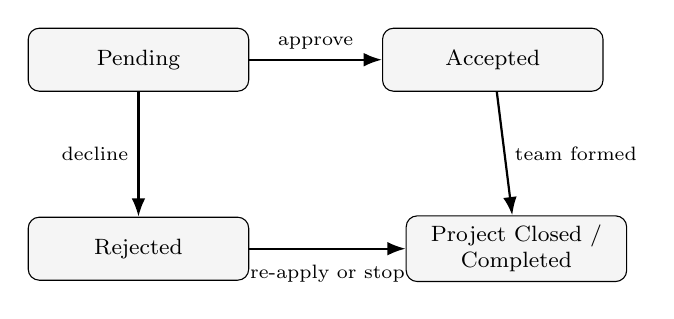
\begin{tikzpicture}[
  every node/.style={font=\footnotesize},
  state/.style={draw, rounded corners, minimum width=2.8cm, minimum height=0.8cm, fill=gray!08, align=center},
  arrow/.style={-Latex, thick}
]
\node[state] (pending) at (0,0) {Pending};
\node[state] (accepted) at (4.5,0) {Accepted};
\node[state] (rejected) at (0,-2.4) {Rejected};
\node[state] (closed) at (4.8,-2.4) {Project Closed /\\Completed};

\draw[arrow] (pending) -- node[above, font=\scriptsize] {approve} (accepted);
\draw[arrow] (pending) -- node[left, font=\scriptsize] {decline} (rejected);
\draw[arrow] (accepted) -- node[right, font=\scriptsize] {team formed} (closed);
\draw[arrow] (rejected) -- node[below, font=\scriptsize, yshift=-2pt] {re-apply or stop} (closed);
\end{tikzpicture}%
}
\caption{State Diagram for Request Lifecycle}
\end{figure}

\section{Functional Requirement of the System (Proposed Modules)}
{\small
\setlength{\tabcolsep}{4pt}
\begin{longtable}{L{0.85in}L{1.45in}L{2.75in}}
\caption{Functional Requirements and Proposed Modules} \\
\toprule
\textbf{Module} & \textbf{Feature} & \textbf{Description} \\
\midrule
\endfirsthead
\toprule
\textbf{Module} & \textbf{Feature} & \textbf{Description} \\
\midrule
\endhead
Authentication & Register, login, token verification & Secure user authentication with password hashing and JWT session control \\
User Profile & Profile create/update & Name, bio, skills, interests, availability, GitHub link, and profile image management \\
Project Posting & Create, view, detail, delete & Lead can post project opportunities, required skills, deadline, and team state \\
Explore & User discovery and filtering & Search teammates by name, skill, and profile availability \\
Request Workflow & Join request and invite & Users apply to teams; leads invite users to their project \\
Team Management & Accept / reject / remove & Lead and admin can manage requests and remove team members where required \\
Chat & Direct conversation & Message exchange with typing state and online presence support \\
Notifications & Event alerts & Request, invite, and message updates with unread state tracking \\
Dashboard & Activity overview & User can see own projects, outgoing requests, incoming requests, and project status \\
Admin & Monitoring and analytics & Admin can review user count, project count, request flow, and recent activities \\
\bottomrule
\end{longtable}
}

\section{Non-functional Requirement}
\begin{itemize}
  \item \textbf{Security:} Password hashing, route protection, and role-aware access control.
  \item \textbf{Reliability:} Deterministic request states, duplicate request protection, and API error handling.
  \item \textbf{Usability:} Clean navigation, mobile responsiveness, and clear call-to-action controls.
  \item \textbf{Performance:} Fast client-side rendering, efficient MongoDB queries, and incremental data loading.
  \item \textbf{Maintainability:} Separated controllers, routes, models, pages, and reusable components.
  \item \textbf{Scalability:} Modular REST endpoints and document-based database suitable for gradual expansion.
\end{itemize}

\chapter{System Design}

\section{Proposed System Architecture}
\begin{figure}[H]
\centering
\resizebox{\linewidth}{!}{%
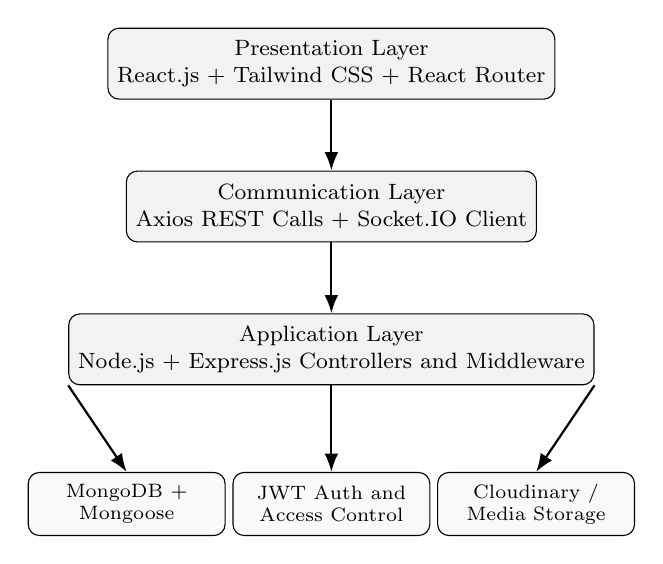
\begin{tikzpicture}[
  every node/.style={font=\footnotesize},
  block/.style={draw, rounded corners, minimum width=5.2cm, minimum height=0.9cm, align=center, fill=gray!10},
  small/.style={draw, rounded corners, minimum width=2.5cm, minimum height=0.8cm, align=center, fill=gray!05, font=\scriptsize},
  arrow/.style={-Latex, thick}
]
\node[block] (client) {Presentation Layer\\React.js + Tailwind CSS + React Router};
\node[block, below=0.9cm of client] (comm) {Communication Layer\\Axios REST Calls + Socket.IO Client};
\node[block, below=0.9cm of comm] (server) {Application Layer\\Node.js + Express.js Controllers and Middleware};
\node[small, below=1.1cm of server, xshift=-2.6cm] (db) {MongoDB +\\Mongoose};
\node[small, below=1.1cm of server] (auth) {JWT Auth and\\Access Control};
\node[small, below=1.1cm of server, xshift=2.6cm] (cloud) {Cloudinary /\\Media Storage};

\draw[arrow] (client) -- (comm);
\draw[arrow] (comm) -- (server);
\draw[arrow] (server.south west) -- (db.north);
\draw[arrow] (server) -- (auth);
\draw[arrow] (server.south east) -- (cloud.north);
\end{tikzpicture}%
}
\caption{Proposed System Architecture}
\end{figure}

\section{Database Table and Schema}

\subsection{Database Schema}
The application uses MongoDB collections to store users, projects, requests, messages, and notifications. Mongoose schemas enforce validation rules and model relations using ObjectId references. This choice is suitable because the project contains semi-structured user profiles, array-based skill lists, and evolving collaboration workflows.

\subsection{Database Table}
{\small
\setlength{\tabcolsep}{4pt}
\begin{longtable}{L{1.1in}L{0.95in}L{2.75in}}
\caption{User Collection Schema} \\
\toprule
\textbf{Field} & \textbf{Type} & \textbf{Description} \\
\midrule
\endfirsthead
\toprule
\textbf{Field} & \textbf{Type} & \textbf{Description} \\
\midrule
\endhead
name & String & Full name of the user \\
email & String & Unique login email \\
password & String & Hashed password stored securely \\
skills & Array[String] & Technical or domain skills \\
interests & Array[String] & Areas of interest such as startups or hackathons \\
bio & String & Short self-description \\
profileImage.url & String & Profile image path or placeholder \\
profileImage.publicId & String & Cloud storage identifier if used \\
githubLink & String & GitHub profile URL \\
availability & String & Availability statement \\
role & String & user or admin \\
bookmarks & Array[ObjectId] & Saved project references \\
createdAt, updatedAt & Date & Automatic timestamps \\
\bottomrule
\end{longtable}
}

{\small
\setlength{\tabcolsep}{4pt}
\begin{longtable}{L{1.1in}L{0.95in}L{2.75in}}
\caption{Project Collection Schema} \\
\toprule
\textbf{Field} & \textbf{Type} & \textbf{Description} \\
\midrule
\endfirsthead
\toprule
\textbf{Field} & \textbf{Type} & \textbf{Description} \\
\midrule
\endhead
title & String & Name of the project \\
description & String & Detailed project summary \\
requiredSkills & Array[String] & Skills required for the project \\
createdBy & ObjectId & User who created the project \\
teamLead & ObjectId & Lead responsible for approval and team control \\
members & Array[ObjectId] & Team members linked to the project \\
status & String & open, in-progress, or closed \\
deadline & Date & Proposed submission or completion date \\
bookmarkedBy & Array[ObjectId] & Users who bookmarked the project \\
createdAt, updatedAt & Date & Automatic timestamps \\
\bottomrule
\end{longtable}
}

{\small
\setlength{\tabcolsep}{4pt}
\begin{longtable}{L{1.1in}L{0.95in}L{2.75in}}
\caption{Request Collection Schema} \\
\toprule
\textbf{Field} & \textbf{Type} & \textbf{Description} \\
\midrule
\endfirsthead
\toprule
\textbf{Field} & \textbf{Type} & \textbf{Description} \\
\midrule
\endhead
sender & ObjectId & User who initiated join request or invite \\
receiver & ObjectId & User who receives the request or invite \\
projectId & ObjectId & Related project reference \\
requestType & String & join or invite \\
status & String & pending, accepted, rejected \\
note & String & Optional textual note \\
createdAt, updatedAt & Date & Automatic timestamps \\
\bottomrule
\end{longtable}
}

{\small
\setlength{\tabcolsep}{4pt}
\begin{longtable}{L{1.1in}L{0.95in}L{2.75in}}
\caption{Message Collection Schema} \\
\toprule
\textbf{Field} & \textbf{Type} & \textbf{Description} \\
\midrule
\endfirsthead
\toprule
\textbf{Field} & \textbf{Type} & \textbf{Description} \\
\midrule
\endhead
sender & ObjectId & User who sends the message \\
receiver & ObjectId & User who receives the message \\
message & String & Message content \\
projectId & ObjectId & Optional project context \\
readAt & Date & Read timestamp if implemented later \\
createdAt, updatedAt & Date & Automatic timestamps \\
\bottomrule
\end{longtable}
}

{\small
\setlength{\tabcolsep}{4pt}
\begin{longtable}{L{1.1in}L{0.95in}L{2.75in}}
\caption{Notification Collection Schema} \\
\toprule
\textbf{Field} & \textbf{Type} & \textbf{Description} \\
\midrule
\endfirsthead
\toprule
\textbf{Field} & \textbf{Type} & \textbf{Description} \\
\midrule
\endhead
userId & ObjectId & User who owns the notification \\
text & String & Human-readable notification body \\
type & String & request, request-update, message, or system \\
isRead & Boolean & Unread state tracking \\
referenceId & ObjectId & Linked record identifier \\
referenceModel & String & Name of the referenced model \\
createdAt, updatedAt & Date & Automatic timestamps \\
\bottomrule
\end{longtable}
}

\section{External Interface Requirement}

\subsection{User Interface}
The user interface follows a responsive single-page application model. Important UI considerations include:
\begin{itemize}
  \item Clear entry points for login, registration, and profile completion.
  \item Feed cards for open project opportunities.
  \item Explore page with teammate discovery and project-based invite action.
  \item Project detail page with full description, team members, request state, and lead actions.
  \item Chat inbox limited to actual conversations, not every system user.
  \item Dashboard for project owners and collaborators to monitor requests and progress.
\end{itemize}

\subsection{Hardware Interface (If Applicable)}
The system does not require specialised hardware. It operates through standard computing devices such as laptops, desktops, or smartphones using a web browser. Optional hardware interaction is limited to file upload devices such as camera-based image capture for profile photos.

\section{Report Design}
Although the platform is primarily interactive, two structured outputs are meaningful for project administration and academic review.

\subsection{Report 1: Project Vacancy Report}
This report presents open projects with title, lead name, required skills, number of current members, and deadline. It can be used by faculty coordinators or hackathon mentors to review ongoing opportunities.

\begin{table}[H]
\centering
\caption{Sample Structure of Project Vacancy Report}
{\small
\setlength{\tabcolsep}{4pt}
\begin{tabularx}{\textwidth}{@{} >{\raggedright\arraybackslash}p{0.17\linewidth} >{\raggedright\arraybackslash}p{0.13\linewidth} X >{\centering\arraybackslash}p{0.09\linewidth} >{\centering\arraybackslash}p{0.11\linewidth} @{}}
\toprule
\textbf{Project Title} & \textbf{Lead} & \textbf{Required Skills} & \textbf{Members} & \textbf{Deadline} \\
\midrule
Find My Teammate & Team Lead Name & React, Node.js, MongoDB & 4 & 30/05/2026 \\
\bottomrule
\end{tabularx}
}
\end{table}

\subsection{Report 2: Team Request Status Report}
This report summarises join requests and invitations with sender, receiver, project title, request type, and current status.

\begin{table}[H]
\centering
\caption{Sample Structure of Team Request Status Report}
{\small
\setlength{\tabcolsep}{4pt}
\begin{tabularx}{\textwidth}{@{} >{\raggedright\arraybackslash}p{0.12\linewidth} >{\raggedright\arraybackslash}p{0.12\linewidth} X >{\centering\arraybackslash}p{0.1\linewidth} >{\centering\arraybackslash}p{0.1\linewidth} @{}}
\toprule
\textbf{Sender} & \textbf{Receiver} & \textbf{Project} & \textbf{Type} & \textbf{Status} \\
\midrule
User A & User B & Find My Teammate & Invite & Pending \\
\bottomrule
\end{tabularx}
}
\end{table}

\chapter{Testing}

\section{Test Cases}
{\small
\setlength{\tabcolsep}{4pt}
\begin{longtable}{C{0.55in}L{1.75in}L{2.35in}C{0.65in}}
\caption{Representative Test Cases} \\
\toprule
\textbf{ID} & \textbf{Test Scenario} & \textbf{Expected Result} & \textbf{Status} \\
\midrule
\endfirsthead
\toprule
\textbf{ID} & \textbf{Test Scenario} & \textbf{Expected Result} & \textbf{Status} \\
\midrule
\endhead
TC-01 & Register with valid details & User account created and token returned & Pass \\
TC-02 & Login with incorrect password & Proper error message is displayed & Pass \\
TC-03 & Update profile with skills and bio & User profile updates successfully & Pass \\
TC-04 & Create a project post & Project appears in dashboard and detail page & Pass \\
TC-05 & Feed excludes own created projects by default & User does not see own post in public feed & Pass \\
TC-06 & Send join request to project & Request record created and notification generated & Pass \\
TC-07 & Invite a teammate from Explore page & Invite request stored with requestType = invite & Pass \\
TC-08 & Accept invitation & Invited user becomes member of the project & Pass \\
TC-09 & Open chat inbox without prior conversation & Inbox remains empty until a conversation starts & Pass \\
TC-10 & Send direct message & Message stored and delivered to receiver in real time & Pass \\
TC-11 & Mark notifications as read & Notification unread count decreases correctly & Pass \\
TC-12 & Remove teammate from project & Team member is removed by project lead/admin & Pass \\
\bottomrule
\end{longtable}
}

\section{Testing Strategy Applied}
The project uses a combination of the following testing strategies:
\begin{enumerate}[label=\arabic*.]
  \item \textbf{Unit-level logic verification:} Controller flows were validated for request, invite, and member-management cases.
  \item \textbf{API testing:} Endpoints were checked using authenticated requests for create, read, update, delete, and role-based access.
  \item \textbf{Integration testing:} Interactions between project creation, request submission, acceptance, and chat/notification generation were validated end to end.
  \item \textbf{UI verification:} Frontend navigation, form submission, feed behaviour, and detail-page routing were tested after each major change.
  \item \textbf{Regression checking:} New fixes such as conversation filtering, own-feed exclusion, and invite acceptance were re-tested to ensure previous features remained functional.
\end{enumerate}

\chapter{Conclusion}
The project \projecttitle\ successfully addresses the practical academic problem of finding the right teammates for project-based work. By combining profile management, skill visibility, opportunity posting, structured request handling, real-time communication, and role-based dashboards, the system converts an unstructured social process into a formal collaborative workflow.

From a technical perspective, the project demonstrates a complete MERN application with reusable frontend components, protected backend routes, schema-driven data modelling, and live communication using web sockets. The completed implementation shows that a carefully designed academic collaboration platform can improve discoverability, reduce coordination delays, and support better project team formation.

The system is also educationally valuable because it consolidates multiple software engineering concepts into one application: database design, authentication, REST API development, state management, modular UI composition, system testing, and documentation.

\chapter{Future Enhancement}
The current version establishes a strong foundation. Future enhancements may include:
\begin{enumerate}[label=\arabic*.]
  \item AI-driven teammate recommendation based on skills, interests, and prior project compatibility.
  \item Video calling and group meeting support for distributed collaboration.
  \item Multi-project team workspaces with shared files and task boards.
  \item GitHub repository linking and automatic contribution statistics.
  \item Email and push notifications for request and message events.
  \item Advanced analytics for project success rates and skill demand trends.
  \item Native Android or cross-platform mobile application.
  \item Faculty approval workflow for official semester project registration.
\end{enumerate}

\chapter{Research Paper}

\section{Proposed Research Paper Title}
\textbf{Find My Teammate: A Skill-Centric MERN Platform for Academic and Startup Collaboration}

\section{Proposed Abstract}
This paper presents \projecttitle, a web-based collaboration platform that improves team formation for academic projects, hackathons, and early-stage startup initiatives. Existing informal approaches to teammate discovery rely heavily on social groups, manual coordination, and fragmented communication tools, which often lead to skill mismatch and delayed execution. The proposed system addresses this gap through a skill-centric workflow that combines profile management, project posting, join requests, teammate invitations, real-time chat, and notification-based coordination. The platform is implemented using the MERN stack with JWT authentication and Socket.IO for real-time capabilities. A modular database schema and role-based API design support maintainability and scalable extension. The paper discusses system design, implementation methodology, and the practical value of consolidating discovery, coordination, and communication in a single academic collaboration environment.

\section{Keywords}
Team discovery, MERN stack, project collaboration, academic platform, real-time chat, skill matching, web application.

\section{Research Contribution}
The proposed research contribution of this project is threefold:
\begin{itemize}
  \item It formalises the workflow of team formation rather than treating it as a purely social process.
  \item It introduces both \textit{join requests} and \textit{lead-driven invitations} in a single project-centric model.
  \item It demonstrates how lightweight real-time communication can be integrated with structured project workflows for academic use.
\end{itemize}

\section{Potential Evaluation Parameters}
The research paper derived from this project can evaluate the system using:
\begin{enumerate}[label=\arabic*.]
  \item Average time required to discover a relevant teammate.
  \item Number of accepted requests and invitations per active project.
  \item User satisfaction regarding interface clarity and communication flow.
  \item Reduction in project team formation delays compared to informal methods.
  \item Technical performance indicators such as API response time and message delivery responsiveness.
\end{enumerate}

\section{Possible Publication Outlets}
The work can be refined for publication in:
\begin{itemize}
  \item National conferences on software engineering and web technologies.
  \item Student research journals focusing on applied computer applications.
  \item Institutional innovation or project compendiums.
\end{itemize}

\chapter{References / Bibliography}

\begin{thebibliography}{99}
\bibitem{reactdocs}
React Documentation.
\newblock \url{https://react.dev/}
\newblock Accessed May 2026.

\bibitem{nodedocs}
Node.js Documentation.
\newblock \url{https://nodejs.org/en/docs}
\newblock Accessed May 2026.

\bibitem{expressdocs}
Express.js Guide.
\newblock \url{https://expressjs.com/}
\newblock Accessed May 2026.

\bibitem{mongodbdocs}
MongoDB Manual.
\newblock \url{https://www.mongodb.com/docs/}
\newblock Accessed May 2026.

\bibitem{mongoosedocs}
Mongoose Documentation.
\newblock \url{https://mongoosejs.com/docs/}
\newblock Accessed May 2026.

\bibitem{socketiodocs}
Socket.IO Documentation.
\newblock \url{https://socket.io/docs/}
\newblock Accessed May 2026.

\bibitem{jwtio}
JWT Introduction.
\newblock \url{https://jwt.io/introduction}
\newblock Accessed May 2026.

\bibitem{owasp}
OWASP Foundation.
\newblock Authentication Cheat Sheet.
\newblock \url{https://cheatsheetseries.owasp.org/}
\newblock Accessed May 2026.

\bibitem{uml}
Object Management Group.
\newblock Unified Modeling Language (UML) Specification.
\newblock \url{https://www.omg.org/spec/UML/}
\newblock Accessed May 2026.

\bibitem{softwareeng}
Roger S. Pressman and Bruce R. Maxim.
\newblock \textit{Software Engineering: A Practitioner's Approach}.
\newblock McGraw-Hill Education.
\end{thebibliography}

\appendix

\chapter{Appendix A: Major REST API Endpoints}
{\small
\setlength{\tabcolsep}{4pt}
\begin{longtable}{C{0.75in}L{1.45in}L{2.8in}}
\toprule
\textbf{Method} & \textbf{Endpoint} & \textbf{Purpose} \\
\midrule
\endfirsthead
\toprule
\textbf{Method} & \textbf{Endpoint} & \textbf{Purpose} \\
\midrule
\endhead
POST & /api/auth/register & Register a new user \\
POST & /api/auth/login & Authenticate existing user \\
GET & /api/auth/me & Get current authenticated user \\
GET & /api/users & Search and list users \\
GET & /api/users/:id & Get user profile and linked projects \\
PUT & /api/users/update & Update user profile \\
PUT & /api/users/bookmarks/:projectId & Toggle bookmarked project \\
GET & /api/users/admin/overview & Admin metrics summary \\
POST & /api/projects/create & Create new project \\
GET & /api/projects & List projects with filters \\
GET & /api/projects/:id & Get project details and requests \\
DELETE & /api/projects/:id & Delete project \\
DELETE & /api/projects/:id/members/:memberId & Remove teammate from project \\
GET & /api/requests & Get requests by view type \\
POST & /api/requests/send & Send join request or project invite \\
PUT & /api/requests/accept & Accept request or invite \\
PUT & /api/requests/reject & Reject request or invite \\
GET & /api/messages & Get conversation list \\
GET & /api/messages/:id & Get direct message thread \\
POST & /api/messages/send & Send a message \\
GET & /api/notifications & Get notifications list \\
PUT & /api/notifications/read-all & Mark all notifications as read \\
PUT & /api/notifications/:id/read & Mark one notification as read \\
\bottomrule
\end{longtable}
}

\chapter{Appendix B: Source Code Structure}
\begin{verbatim}
find-my-teammate/
|-- client/
|   |-- src/
|   |   |-- components/
|   |   |-- context/
|   |   |-- hooks/
|   |   |-- pages/
|   |   |-- services/
|   |   `-- utils/
|   |-- package.json
|   `-- vite.config.js
|-- server/
|   |-- config/
|   |-- constants/
|   |-- controllers/
|   |-- middleware/
|   |-- models/
|   |-- routes/
|   |-- sockets/
|   |-- .env
|   |-- package.json
|   `-- server.js
|-- package.json
`-- README.md
\end{verbatim}

\chapter{Appendix C: Sample Environment Configuration}
\begin{verbatim}
# server/.env
PORT=5000
MONGO_URI=mongodb://127.0.0.1:27017/find-my-teammate
JWT_SECRET=replace_with_secure_secret
CLIENT_URL=http://localhost:5173,http://localhost:5174
CLOUDINARY_CLOUD_NAME=
CLOUDINARY_API_KEY=
CLOUDINARY_API_SECRET=

# client/.env
VITE_API_URL=http://localhost:5000/api
\end{verbatim}

\end{document}
